% Created 2023-09-15 Fri 21:54
% Intended LaTeX compiler: pdflatex
\documentclass[11pt]{article}
\usepackage[utf8]{inputenc}
\usepackage[T1]{fontenc}
\usepackage{graphicx}
\usepackage{longtable}
\usepackage{wrapfig}
\usepackage{rotating}
\usepackage[normalem]{ulem}
\usepackage{amsmath}
\usepackage{amssymb}
\usepackage{capt-of}
\usepackage{hyperref}
\usepackage{graphicx, siunitx}
\graphicspath{ {./images/} }
\author{Hankertrix}
\date{\today}
\title{Chemical Kinetics Cheat Sheet}
\hypersetup{
 pdfauthor={Hankertrix},
 pdftitle={Chemical Kinetics Cheat Sheet},
 pdfkeywords={},
 pdfsubject={},
 pdfcreator={Emacs 29.1 (Org mode 9.6.6)}, 
 pdflang={English}}
\begin{document}

\maketitle
\setcounter{tocdepth}{2}
\tableofcontents

\newpage

\section{Definitions}
\label{sec:org29eaa41}

\subsection{Reaction rate}
\label{sec:orgd6ee90b}
Either the \textbf{increase} in the concentration of a product per unit time or the \textbf{decrease} in the concentration of a reactant per unit time.
\\[0pt]

General reaction:
\[aA + bB \rightarrow dD + eE\]

\[\text{Rate of reaction} = - \frac{1}{a}\frac{d[A]}{dt} = - \frac{1}{b}\frac{d[B]}{dt} = - \frac{1}{d}\frac{d[D]}{dt} = - \frac{1}{e}\frac{d[E]}{dt}\]

\subsubsection{Example}
\label{sec:orga8845ac}

\[2N_2O_5 (g) \rightarrow 4 NO_2 (g) + O_2 (g)\]

\[\text{Rate of reaction} = \frac{1}{2}\frac{d[N_2O_5]}{dt} = \frac{1}{4}\frac{d[NO_2]}{dt} = \frac{d[O_2]}{dt}\]
\[\text{Rate of reaction} = k[N_2O_5]^2\]
\[\text{Rate of consumption of reactant} = -\frac{d[N_2O_5]}{dt} = 2 \cdot k[N_2O_5]^2\]
\[\text{Rate of formation of product} = -\frac{d[NO_2]}{dt} = 4 \cdot k[N_2O_5]^2\]
\[\text{Rate of formation of product} = -\frac{d[O_2]}{dt} = k[N_2O_5]^2\]

\subsection{Rate law}
\label{sec:orge9546e5}
The rate law is an equation that shows the dependence of the reaction rate on the concentration of each reactant.

\[aA + bB \rightarrow \text{ Products}\]
\[\text{Rate} \propto [A]^m[B]^n\]
\[\text{Rate} = k[A]^m[B]^n\]

\(k\) is the \textbf{rate constant}.
\\[0pt]

The values of the exponents in the rate law must be \textbf{determined experimentally}. They cannot be deduced from the stoichiometry of the reaction.
\\[0pt]

\subsubsection{Units of the rate constant \(k\)}
\label{sec:org96baf3b}

The units of \(k\) must be determined based on the order of the reaction. For example, given a third order reaction:

\[2NO(g) + O_2(g) \rightarrow 2NO_2 (g)\]
\[\text{Rate} = k[NO]^2[O_2]\]

Units of \(k\) for this third-order reaction:
\[k = \frac{\text{Rate}}{[NO^2][O_2]} = \frac{\frac{M}{s}}{M^2 \cdot M} = \frac{1}{M^2 s}\]

\subsubsection{The rate constant \(k\) is dependent on temperature}
\label{sec:org418defb}
The \textbf{rate constant} \(k\) is dependent on temperature and the \textbf{rate of reaction} usually \textbf{increases} when the \textbf{temperature increases}.

\subsection{Half-life}
\label{sec:org050967b}
The half-life is the \textbf{time} required for the reactant concentration to drop to \textbf{one-half} of its initial value.

\subsection{Transition state}
\label{sec:orgd1b4643}
The transition state is the configuration of atoms at the maximum in the potential energy profile. This is also called the activated complex.

\subsection{Collision theory}
\label{sec:org1bb204a}
Collision theory states that as the average \textbf{kinetic energy} increases, the average \textbf{molecular speed} increases and thus the \textbf{collision rate} increases.

\newpage

\subsection{Arrhenius equation}
\label{sec:orgfdc35e0}
\[k = Ae^{\frac{-E_a}{RT}}\]

Where:
\begin{itemize}
\item \(k\) is the rate constant
\item \(A\) is the collision frequency factor
\item \(E_a\) is the activation energy
\item \(R\) is the gas constant
\item \(T\) is the temperature in Kelvin (\(\unit{K}\))
\end{itemize}

\subsubsection{Using the Arrhenius equation}
\label{sec:org2095940}
\[\ln (k) = \ln (A) + \ln \left[e^{\frac{-E_a}{RT}} \right]\]
\[\ln (k) = \ln (A) - \frac{-E_a}{RT}\]
\[\ln (k) = \frac{-E_a}{R} \frac{1}{T} + \ln (A) \text{ which is in the form: } y = mx + c\]
\\[0pt]

So, we get:
\[\ln \left( \frac{k_2}{k_1} \right) = \frac{-E_a}{R} \left( \frac{1}{T_2} - \frac{1}{T_1} \right)\]

Plotting the graph of \(\ln(k)\) versus \(\frac{1}{T}\) gives a straight line graph with a \textbf{slope (gradient)} of \(\frac{-E_a}{R}\).

\newpage

\subsubsection{Which gas constant \((R)\) value to use?}
\label{sec:org4f4a121}
The gas constant can be either:

\begin{itemize}
\item \(R\) value: 8.314 \\[0pt]
Units: \(\unit{J.K^{-1}.mol^{-1}}, \ \unit{m^3.Pa.K^{-1}.mol{^-1}}\)

\item \(R\) value: 0.0821 \\[0pt]
Units: \(\unit{L.atm.K^{-1}.mol^{-1}}\)
\end{itemize}

\[\ln \left( \frac{k_2}{k_1} \right) = \frac{-E_a}{R} \left( \frac{1}{T_2} - \frac{1}{T_1} \right)\]
\\[0pt]

For the term \(\frac{-E_a}{R}\), the final units should be \(\unit{K}\).
\\[0pt]

If \(R = \qty{8.314}{\unit{J.K^{-1}.mol^{-1}}}\), the units for \(E_a\) should be \(\unit{J.mol^{-1}}\).

If \(R = \qty{0.0821}{\unit{L.atm.K^{-1}.mol^{-1}}}\), the units for \(E_a\) should be \(\unit{L.atm.mol^{-1}}\).

\subsection{Elementary reaction (elementary step)}
\label{sec:orgbd073eb}
A single step in a reaction mechanism. An elementary reaction describes an individual molecular event.

\subsection{Overall reaction}
\label{sec:orgfb905db}
The overall reaction described the reaction stoichiometry and is a summation of elementary reactions.

\subsection{Reaction mechanism}
\label{sec:orgac190c5}
The reaction mechanism is a sequence of reaction steps that describes the pathway from reactants to products.

\subsubsection{Example}
\label{sec:orgfa4b409}
\[NO_2 (g) + NO_2 (g) \rightarrow NO (g) + NO_3 (g) \textbf{ Elementary reaction}\]
\[NO_3 (g) + CO (g) \rightarrow NO_2 (g) + CO_2 (g) \textbf{ Elementary reaction}\]
\hrule
\[NO_2 (g) + CO (g) \rightarrow NO (g) + CO_2 (g) \textbf { Overall reaction}\]

\subsection{Molecularity}
\label{sec:org53db2d3}
Molecularity is a classification of an elementary reaction based on the number of molecules or atoms on the reactant side of the chemical equation.

\subsubsection{Unimolecular reaction}
\label{sec:org8dae514}
\[O_3^* (g) \rightarrow O_2 (g) + O (g)\]
\[\text{Rate} = k[O_3]\]

\subsubsection{Bimolecular reaction}
\label{sec:org42c9aeb}
\[O_3 (g) + O (g) \rightarrow 2O_2 (g)\]
\[\text{Rate} = k[O_3][O]\]

\subsubsection{Termolecular reaction}
\label{sec:org9510b29}
\[O (g) + O (g) + M (g) \rightarrow O_2 (g) + M (g)\]
\[\text{Rate} = k[O]^2[M]\]

\subsection{Rate-determining step}
\label{sec:org9d1f540}
The rate-determining step is the \textbf{slow step} in a reaction mechanism since it acts as a bottleneck and limits the rate at which reactants can be converted to products.

\newpage

\subsection{Catalyst}
\label{sec:orgc3db480}
A catalyst is a substance that increases the rate of a reaction without itself being consumed in the reaction. A catalyst is used in one step and regenerated in a later step.

\subsubsection{Example}
\label{sec:orga61bc14}
\(I^- (aq)\) is acting as a catalyst in the reaction below as it is regenerated and not used up:

\[H_2 O_2 (aq) + I^- (aq) \rightarrow H_2O (l) + IO^- (aq) \textbf{ Rate-determining step}\]
\[H_2 O_2 (aq) + IO^- (aq) \rightarrow H_2O (l) + O^2 (g) + I^- (aq) \textbf{ Fast step}\]
\hrule
\[2H_2O_2 (aq) \rightarrow 2H_2O (l) + O_2 (g) \textbf{ Overall reaction}\]
\\[0pt]

Since the catalyst is involved in the \textbf{rate-determining step}, it often appears in the rate law. The rate law for the reaction above is:
\[\text{Rate} = k[H_2O_2][I^-]\]

\subsubsection{Effect of a catalyst}
\label{sec:orgf4ef968}
A catalyst will \textbf{decrease} the \textbf{activation energy} (\(E_a\)) of a reaction and there will usually be \textbf{two transition states} in the reaction, which means 2 humps in the energy level diagram for the reaction. The first hump will be \textbf{larger} than the second one as the first hump represents the activation energy for the reaction.

\subsection{Homogeneous catalyst}
\label{sec:org8f8dcbb}
A homogeneous catalyst is a catalyst that exists in the \textbf{same phase} as the reactants.

\newpage

\subsection{Heterogeneous catalyst}
\label{sec:org26f8a45}
A catalyst that exists in a \textbf{different phase} from that of the reactants.

\subsubsection{Example mechanism}
\label{sec:org24b3b06}
Using a metal catalyst for the reaction between \(H_2\) and \(C_2H_4\):

\begin{enumerate}
\item \(H_2\) and \(C_2H_4\) are adsorbed on the metal surface.
\item The \(H-H\) bond breaks as \(H\)-metal bonds form, and the \(H\) atoms move about on the surface.
\item One \(H\) atom forms a bond to a \(C\) atom of the adsorbed \(C_2H_4\) to give a metal-bonded \(C_2H_5\) group. A second \(H\) atom bonds to the \(C_2H_5\) group.
\item The resulting \(C_2H_6\) molecule is desorbed from the surface.
\end{enumerate}

\section{Characteristics of zeroth, first, and second-order reactions}
\label{sec:org274bf5e}

\[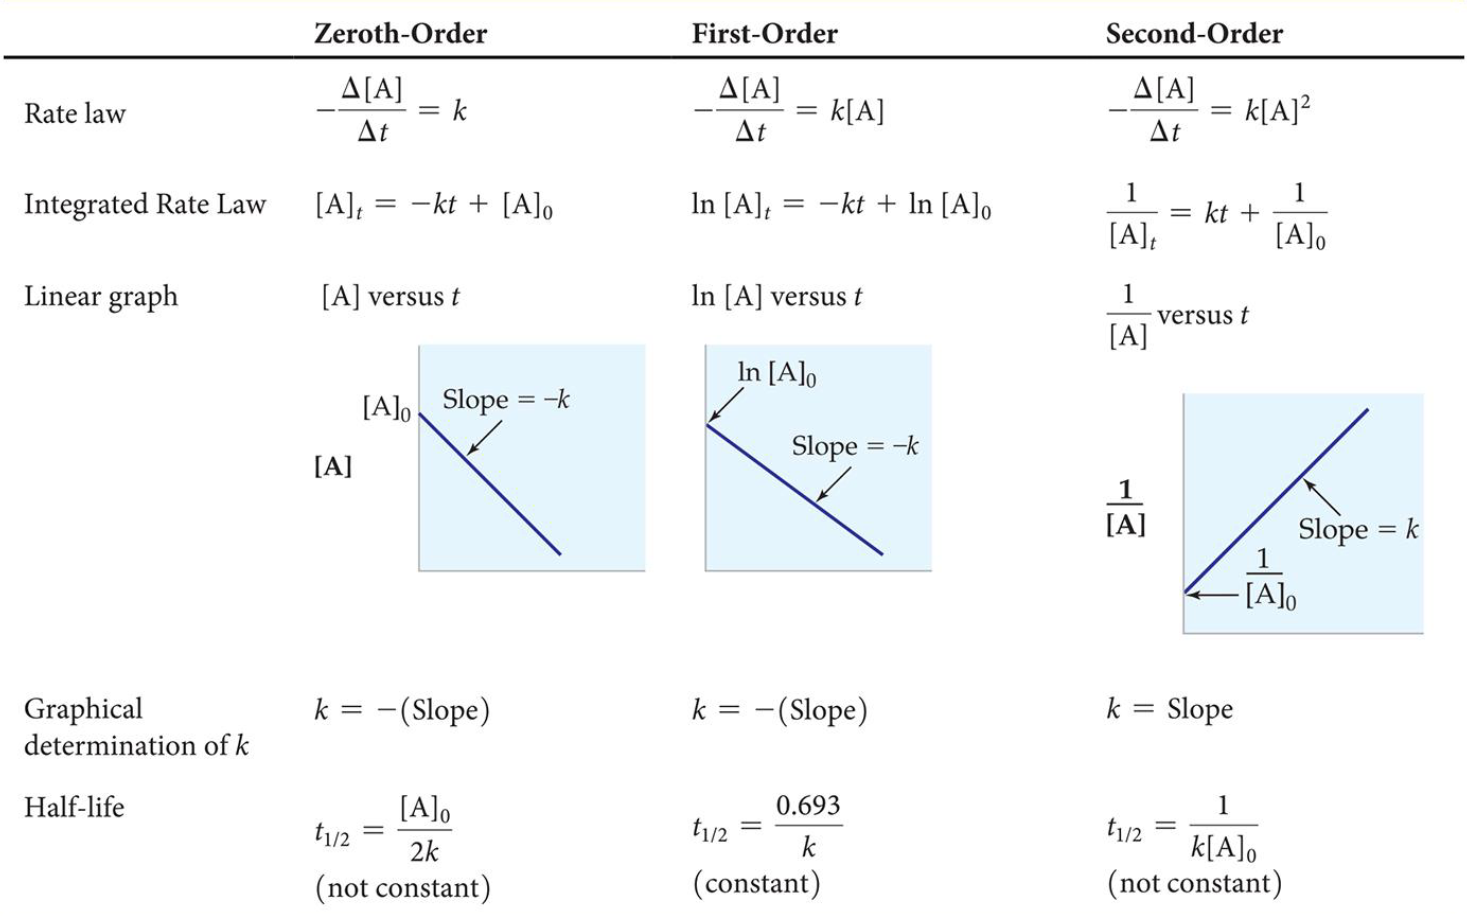
\includegraphics[width = \textwidth]{characteristics}\]

\newpage

\section{Zeroth-order reactions}
\label{sec:org5a1d356}
For a zeroth-order reaction, the rate is \textbf{independent} of the concentration of the reactant.

\[A \rightarrow \text{ Products}\]
\[\text{Rate} = k[A]^0 = k\]
\[- \frac{\Delta [A]}{\Delta t} = k\]

The \textbf{integrated rate law} for a zeroth-order reaction is:
\[[A]_t = -kt + [A]_0, \text{ which is in the form: } y = mx + c\]

Where \([A]_t\) is the concentration of \(A\) at time \(t\) and \([A]_0\) is the initial concentration of \(A\).
\\[0pt]

A plot of \([A]\) versus \textbf{time} gives a straight-line graph and the \textbf{slope (gradient)} will be \(-k\).

\subsection{Example}
\label{sec:orgc40524b}
\[2NH_3 (g) \rightarrow N_2 (g) + 3H_2 (g)\]
\[\text{Rate} = k[NH_3]^0 = k\]

\subsubsection{Explanation (not very important)}
\label{sec:org348f21b}
Most of the \(NH_3\) molecules are in the gas phase above the surface and are unable to react. As the \(NH_3\) molecules on the surface decompose, they are replaced by molecules form the gas phase, so the number of \(NH_3\) molecules on the surface remains constant. Because only the \(NH_3\) molecules on the surface react under these conditions, the reaction rate is independent of the total concentration of \(NH_3\).

\newpage

\section{First-order reaction}
\label{sec:org646d0e9}
\[A \rightarrow \text{ Products}\]
\[\text{Rate} = k[A]\]
\[- \frac{\Delta [A]}{\Delta t} = k[A]\]

Deriving the \textbf{integrated rate law}:
\[\ln \left( \frac{[A]_t}{[A]_0} = -kt \right)\]
\[\ln [A]_t - \ln [A]_0 = -kt\]

Hence, the \textbf{integrated rate law} is:
\[\ln [A]_t = -kt + \ln [A]_0, \text{ which is in the form: } y = mx + c\]
\[[A]_t = e^{-kt} + [A]_0\]

Where \([A]_t\) is the concentration of \(A\) at time \(t\) and \([A]_0\) is the initial concentration of \(A\).
\\[0pt]

A plot of \(ln[A]\) versus \textbf{time} gives a straight-line graph and the \textbf{slope (gradient)} will be \(-k\).

\subsection{Half-life}
\label{sec:orgc57715b}

Finding the half life of a first-order reaction:
\[A \rightarrow \text{ Products}\]
\[\text{Rate} = k[A]\]
\[\ln \left( \frac{[A]_t}{[A]_0} = -kt \right)\]

When \(t = t_{\frac{1}{2}}\) and \([A]_{t_{\frac{1}{2}}} = \frac{[A]_0}{2}\):
\[\ln \frac{1}{2} = -kt_{\frac{1}{2}}\]

Hence, the half-life of a first-order reaction is:
\[t_{\frac{1}{2}} = \frac{\ln 2}{k}\]

The half-life of a first-order reaction is \textbf{independent} of the initial concentration. Each successive half-life is an equal period of time.


\section{Second-order reaction}
\label{sec:org7a489fd}
\[A \rightarrow \text{ Products}\]
\[\text{Rate} = k[A]^2\]
\[- \frac{\Delta [A]}{\Delta t} = k[A]^2\]

The \textbf{integrated rate law} of a second-order reaction is:
\[\frac{1}{[A]_t} = kt + \frac{1}{[A]_0} \text{ which is in the form: } y = mx + c\]

Where \([A]_t\) is the concentration of \(A\) at time \(t\) and \([A]_0\) is the initial concentration of \(A\).
\\[0pt]

A plot of \(ln[A]\) versus \textbf{time} gives a curve. However, plotting \(\frac{1}{[A]}\) versus \textbf{time} gives a straight-line graph with the \textbf{slope (gradient)} will be \(k\).

\subsection{Half-life}
\label{sec:org48cc9c2}

Finding the half life of a second-order reaction:
\[A \rightarrow \text{ Products}\]
\[\text{Rate} = k[A]\]
\[\frac{1}{[A]_t} = kt + \frac{1}{[A]_0}\]

When \(t = t_{\frac{1}{2}}\) and \([A]_{t_{\frac{1}{2}}} = \frac{[A]_0}{2}\):
\[\frac{2}{[A]_0} = kt_{\frac{1}{2}} + \frac{1}{[A]_0}\]

Hence, the half-life of a second-order reaction is:
\[t_{\frac{1}{2}} = \frac{1}{k[A]_0}\]

For a second-order reaction, the half-life is \textbf{dependent} on the initial concentration. Each successive half-life is \textbf{twice} as long as the preceding one.
\end{document}